\begin{surferPage}[Sextic (30 Cusps)]{The Barth Sextic with 30 Cusps}
    %After Wolf Barth had constructed the sextic with the maximum possible
		Nakon \v{s}to je Wolf Barth konstruirao sekstiku s najve\'{c}im mogu\'{c}im brojem singulariteta
    %number of singularities, $65$ (see another surface in this gallery) and
		$65$ (pogledajte neku drugu plohu u ovoj galeriji) i nakon \v{s}to su dva njegova doktoranda
    %two of his Ph.D.\ students had also constructed new world record surfaces
		tako\dj{}er konstruirala nove plohe za svjetski rekord,
    %for higher degrees, he started to consider the question on the maximum
		za vi\v{s}i stupanj Barth je po\v{c}eo razmatrati pitanje najve\'{c}eg 
    %number of cusps on surfaces of a given degree.
		broja \v{s}iljaka na plohi danog stupnja.

   %Barth's construction of the sextic with $65$ singularities of type
	Barthova kostrukcija sekstike sa $65$ singulariteta tipa
    %$A_1^{+-}$ (double cones) can be adapted to cusps, this yields $30$ of
		$A_1^{+-}$ (dvostruki konus) mo\v{z}e se prilagoditi \v{s}iljcima, dobivamo ih $30$
    %them: 
    \[P_6 - \alpha \cdot K^3=0,\]
 % where $P_6$ are the same symmetry planes of the icosahedron as in the
gdje su $P_6$ iste ravnine simetrije ikosaedra kao u
    %other Barth Sextic. As before $K$ is
		drugoj Barthovoj sekstici. Kao prije $K$ je 
    %again the equation of a unit sphere:
		jednad\v{z}ba jedini\v{c}ne sfere:
    \vspace*{-0.4em}
    \begin{center}
      \begin{tabular}{c@{\ }c@{\ }c@{\ }c}
        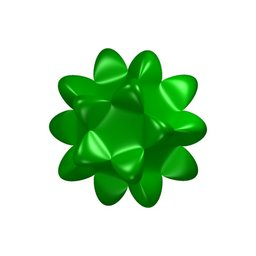
\includegraphics[height=1.2cm]{./../../common/images/barthsextic_30A2}
        &
        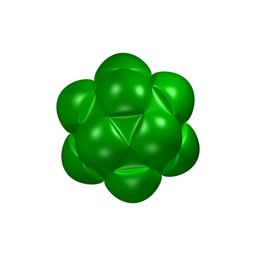
\includegraphics[height=1.2cm]{./../../common/images/barthsextic_30A2_3}
        &
        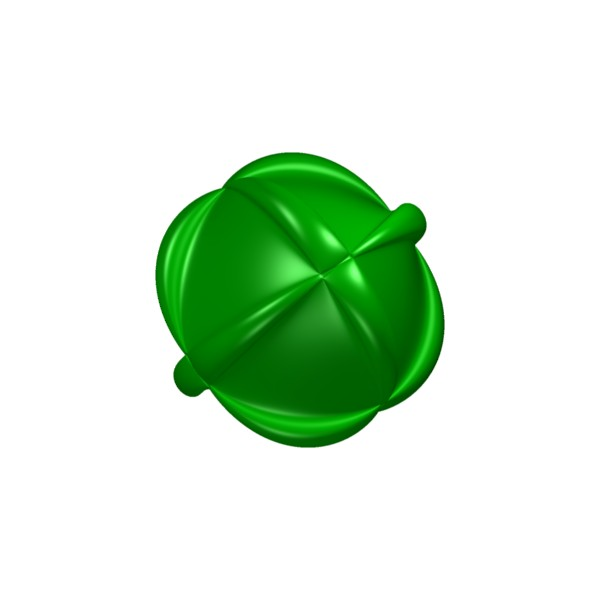
\includegraphics[height=1.2cm]{./../../common/images/barthsextic_30A2_5}
        &
        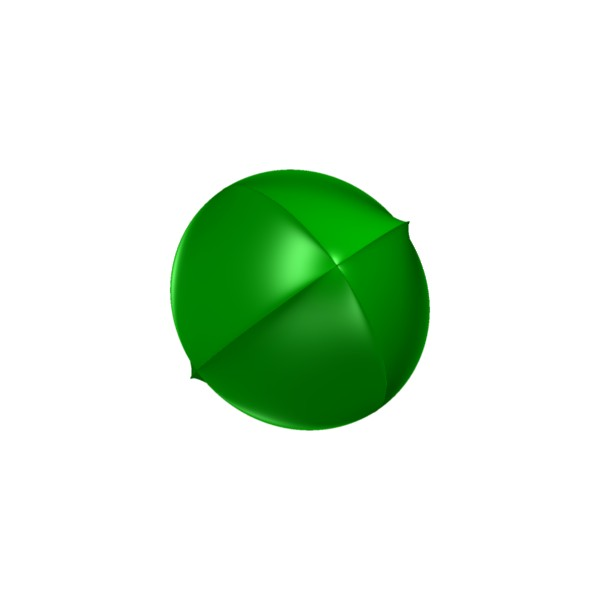
\includegraphics[height=1.2cm]{./../../common/images/barthsextic_30A2_6}
      \end{tabular}
    \end{center}    
    \vspace*{-0.3em}
     %This is the current world record for the maximum number of real cusps on
    %sextics, for complex cusps, it is $36$.
		Ovo je trenuta\v{c}ni svjetski rekord u najve\'{c}em broju realnih \v{s}iljaka na sekstikama. Za kompleksne sekstike rekord je $36$.
\end{surferPage}
